\documentclass{article}
\usepackage[utf8]{inputenc}
\usepackage[margin=1in]{geometry}
\usepackage{indentfirst}
\usepackage{url}
\usepackage{graphicx}
\usepackage{float}
\usepackage{caption}
\usepackage{subcaption}

\title{Everything and More About Protein Classification}
\author{Christopher Mertin}
\date{October 25, 2015}

\begin{document}

\maketitle

To determine the work we did, this paper outlines all of the current information we have and the conclusions we've made, instead of speaking in the first person. Mainly so that we can just copy and paste this bad boy into our final paper. Some of these sections are not filled out as much as we'd like for our paper, but we only did some brief looking at the sections and will be finishing them before the final paper. The topics that need to be covered in this paper are: 
\begin{itemize}
\item The progress you have made towards your goal. (This can not be just “We collected data”.) (50\%)
\item Details of your plan for rest of the semester (30\%)
\item Pointers to literature (20\%)
\end{itemize}


\section*{Introduction}

Machine learning can be used to predict which family a protein chain belongs to. For protein chains, there are only a finite domain of three-dimensional structures embedded in most proteins. By using this domain of structures and identifiable sequence patterns, machine learning techniques should be able to be used to classify the proteins into their respective families. 

For these classifications, different machine learning techniques can be used to classify the data. Below, the ideas of different algorithms are explored and discussed, to determine which of them are viable candidates. Of these algorithms, any of which are viable candidates will be utilized in the final project and the accuracy and efficiency of each of the algorithms will be noted. 

Following this, the data needs to be understood as well before these algorithms can be tried. So the last section looks and references to the locations of this protein data, and how the data is stored. That way it can be parsed and used with the algorithms.

\section*{Protein Classification}

Proteins are molecules responsible for many biological processes in a cell, and they consist of mostly {\em amino acids}. Depending on the sequence of the amino acids depends on the properties that a protein chain has and the interactions and the processes that they're important for.

Proteins fold in 3-dimensions, which means that some are very similar. Therefore, by being able to classify the proteins and determine which ones are similar, it can help determine which ones are important in biological processes. For example, if a new protein is found and it is not understood of its purpose and what interactions it makes, if it falls in a family of proteins that is well known, it will give a good indication of what types of processes that protein can cause to happen in the cell.

There are two ways in which proteins can be classified. The first way is by their sequence, while the second is by their structural similarity. These classifications can be from the {\em families} of which the proteins belong, the {\em domains} they contain, and the {\em sequence features} they possess. 

\subsection*{Families}

A protein family is a group of proteins that come from the same evolutionary chain, which is reflected in their functions, sequences, and structure \cite{EBI}. This is very similar to the evolutionary chain seen in evolutionary biology and can be thought of as the same thing. Figure~\ref{fig:family1} shows an example of how these protein family trees are defined.

\begin{figure}[!h]
\centering
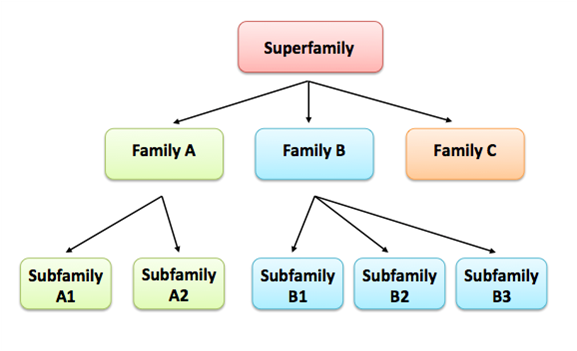
\includegraphics[width=.5\textwidth]{family1.png}
\caption{Pseudo protein family hierarchical tree structure \cite{EBI}}
\label{fig:family1}
\end{figure}

In Figure~\ref{fig:family1}, the term {\em superfamily} denotes the larger group of those proteins which are distantly related and {\em subfamily} denotes small groups of closely related proteins that evolved from a common ancestor. This can be taken to a real-world example with G protein-coupled receptors (GPCRs) in Figure~\ref{fig:family2}.

\begin{figure}[!h]
\centering
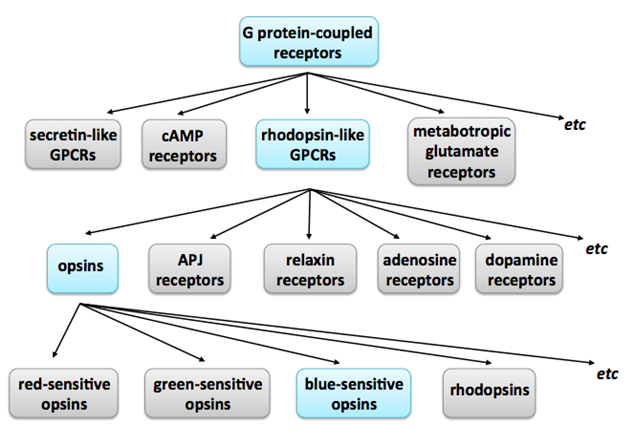
\includegraphics[width=.5\textwidth]{family2.png}
\caption{Example protein family tree for GPCRs \cite{EBI}}
\label{fig:family2}
\end{figure}

GPCRs are a large group of proteins with many different functions in a wide range of biological processes. At the superfamily level, the level that encompasses all GCPRs, two major properties are shared: they have seven transmembrain domains and they interact with specialized proteins (called G proteins) to influence intracellular pathways after binding {\em extracellular signals}. This variety can easily be seen in the family tree in Figure~\ref{fig:family2} as there are many nodes in the tree. If a certain protein family was being looked for such as {\em blue-sensitive opsins}, which are important for photoreceptors, you could easily traverse the tree, as is shown in blue.
\newpage

\subsection*{Domains}

Domains are distinct functional and/or structural units in a protein. Domains of a protein are responsible for a particular function or interaction that the protein has, which contributes to its overall function. Domains exist in a large variety of biological contexts, where even similar domains can cause the protein to have different functions.

For example, Source Homology 3 (SH3) Domains are small domains of around 60 amino acid residues are involved in protein-protein interactions \cite{SH3}. They have been found in proteins of signaling pathways in the cytoskeleton, the Ras protein, and others. SH3 domains have a characteristic structure to them which allows them to be identified, and they occur in a diverse range of proteins with different properties, which can be seen in Figure~\ref{fig:SH3struct}. Proteins can also have multiples of a domain, for example the cytoplasmic protein Nck is described in Figure~\ref{fig:multSH3}.

\begin{figure}[h!]
\centering
\begin{minipage}{.5\textwidth}
  \centering
  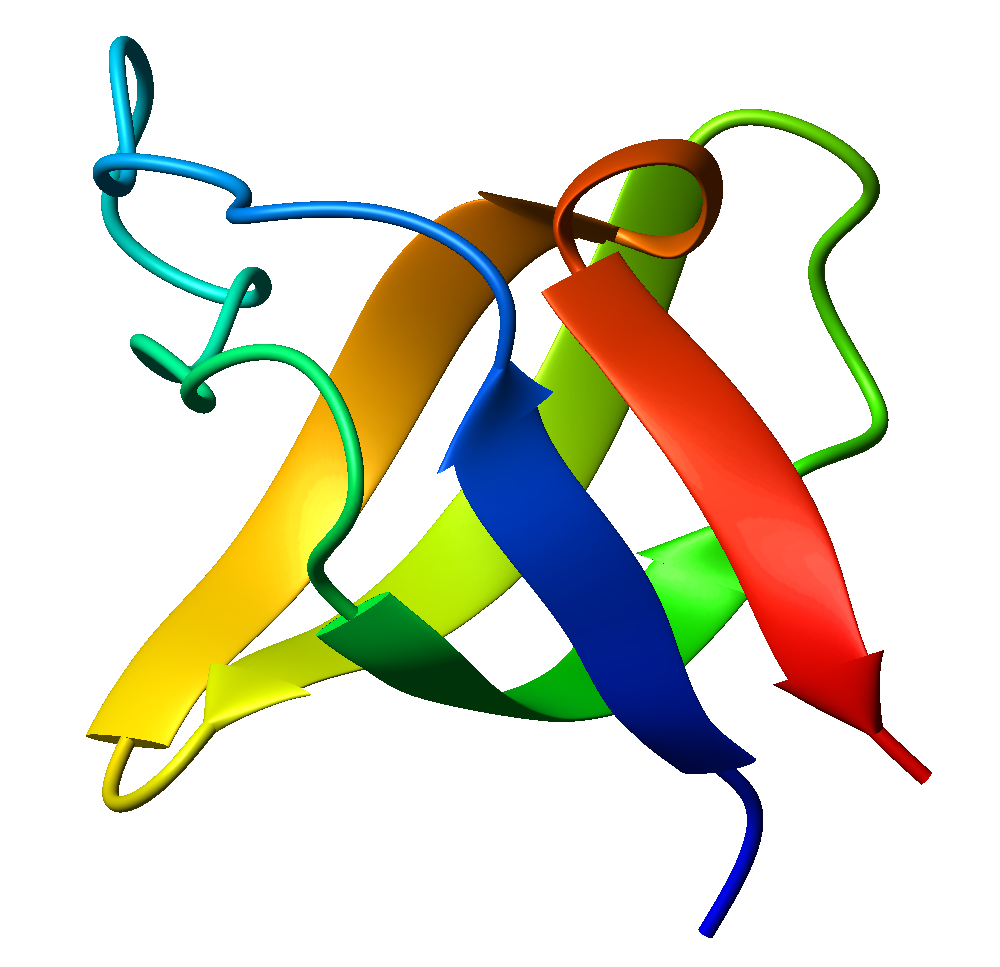
\includegraphics[width=.65\linewidth]{SH3.png}
  \captionof{figure}{Characteristic structure of SH3 domain \cite{SH3}}
  \label{fig:SH3struct}
\end{minipage}%
\begin{minipage}{.5\textwidth}
  \centering
  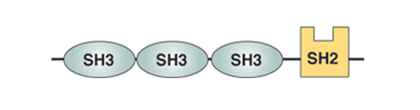
\includegraphics[width=\linewidth]{multsh3.png}
  \captionof{figure}{Domain decomposition of Nck protein \cite{EBI}}
  \label{fig:multSH3}
\end{minipage}
\end{figure}

Individual domains have specific functions, such as binding a particular molecule, being a catalyst in certain reactions, etc, and together they define the function of the protein. For example, as in Figure~\ref{fig:multidomain} it shows the different types of domains in Phospholipase D1, which is an important enzyme. It shows the domains in it and specifically links to the functions that they allow the enzymes to perform.

\begin{figure}[h!]
\centering
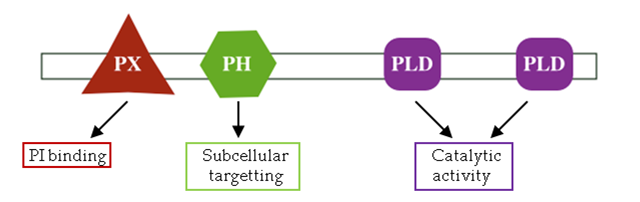
\includegraphics[width=.75\textwidth]{multidomain.png}
\caption{Domain composition of Phospholipase D1 \cite{EBI}}
\label{fig:multidomain}
\end{figure}

\subsubsection*{Family and Domain Protein Classification}

A problem with family classifications based only on family and domains is that it is not always straightforward and can overlap, since proteins are sometimes assigned to families by the domains that they contain. An example in protein classification based on these properties can be found below.

Regulator of G-protein signalling (RGS) domains are proteins that activate GTPases, and are found in sequences that belong to the RGS protein family. However, as can be seen in Figure~\ref{fig:RGSSort}, RGS domains can be found in other families as well, so classifying just based on these methods is not the best choice of action.

\begin{figure}[h!]
\centering
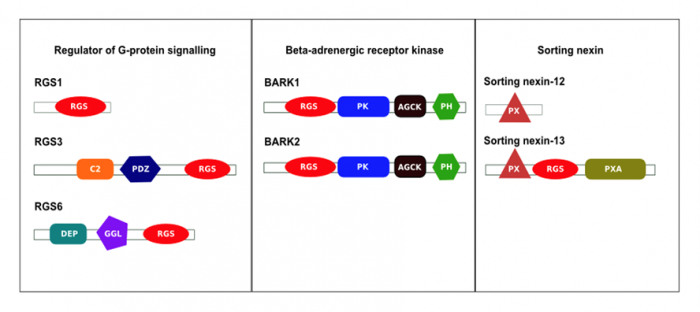
\includegraphics[width=.75\textwidth]{RGSSort.png}
\caption{Example of family classifications which more than one contain the RGS Domain \cite{EBI}}
\label{fig:RGSSort}
\end{figure}

\subsection*{Sequence Features}

Sequence features are a group of amino acids that give the protein certain characteristics which could be useful to its overall function. Some features include

\begin{itemize}
\item {\bf Action Sites:} Contains amino acids involved in catalytic activity. For example, the enzyme lipase, which catalyzes the formation and hydrolysis of fats, has two amino acid residues that are essential for its catalytic activity.
\item {\bf Binding Sites:} Containing amino acids that are directly involved in binding molecules or ions, like the iron-binding site of hemoglobin
\item {\bf Post-Translational Modification (PTM) Sites:} Contain residues known to be chemically modified (phosphorylated, palmitoylated, acetylated, etc) after the process of protein translation.
\item {\bf Repeats:} Typically short amino acid sequences that are repeated within a protein, and may confer binding or structural properties upon it.
\end{itemize}

A pictorial representation of Sequence Features can be seen in Figure~\ref{fig:seq-features}, which shows how they are physically arranged. 

\begin{figure}[h!]
\centering
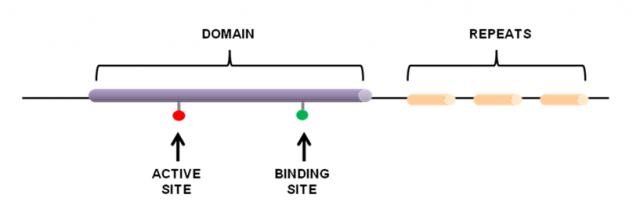
\includegraphics[width=.75\textwidth]{sequencefeatures.png}
\caption{Graphical representation of repeats, domains, and sites on a protein sequence}
\label{fig:seq-features}
\end{figure}

\subsection*{Protein Signatures}

In order to classify proteins into families and to predict the presence of domains or sequence features, {\em protein signatures} have to be used to help classify the proteins. There are many models that are out there to do this, but the most na\"{i}ve approach starts with multiple sequence alignment of proteins sharing a set of characteristics (e.g. belonging to the same family for sharing a domain). When building the initial model, the level of amino acid conversion at different positions in the alignment is taken into account. This model that is made is then searched over the database in an iterative manner, refining the model as more distantly related sequences in the database are identified. 

There are four different approaches that can be used to generate signatures:

\begin{itemize}
\item Patterns
\item Profiles
\item Fingerprints
\item Hidden Markov Models (HMMs)
\end{itemize}

Each of these starts with a protein multiple sequence alignment, and can focus on a single conserved sequence region (known as a {\em motif}), multiple conserved motifs, or the full alignment of the entire protein or a particular {\em domain}. Figure~\ref{fig:motifmethods} shows different techniques that can be used to build these signatures.

\begin{figure}[h!]
\centering
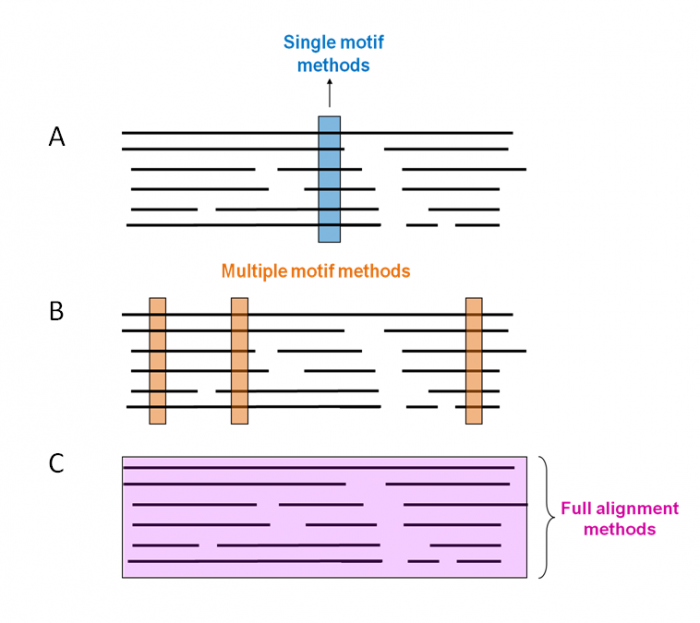
\includegraphics[width=.75\textwidth]{motifmethods.png}
\caption{Different strategies on building signatures. Protein multiple sequence alignments are represented by black lines. (A) Single Motif Method, (B) Multiple Motif Method, (C) Full Alignment Method.}
\label{fig:motifmethods}
\end{figure}

\subsubsection*{Patterns}

Many important sequence features, such as binding sites or the active sites of enzymes, consist of only a few amino acids that are essential for protein function. Patterns are very good at recognising such features. They are built by identifying these regions in multiple sequence alignments. The pattern of conservation within the sequence feature is then modelled as a regular expression, as shown in Figure~\ref{fig:regex}. An example database that uses this is PROSITE.

\begin{figure}
\centering
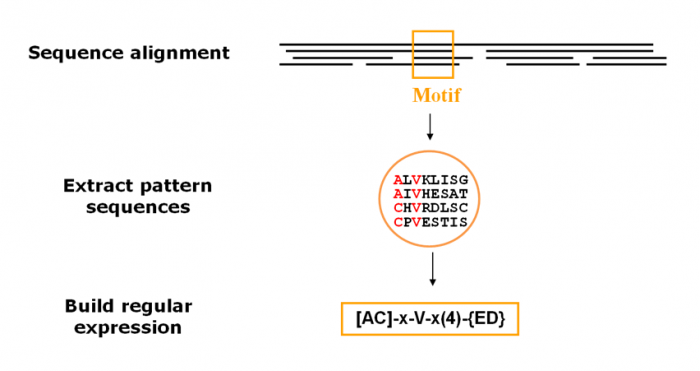
\includegraphics[width=.75\textwidth]{regex.png}
\caption{When creating patterns, as conserved {\em motif} is used to build a regular expression. The pattern illustrated here is translated as: [Ala or Cys]-any-Val-any-any-any-any-[any but Gly or Asp] \cite{EBI}.}
\label{fig:regex}
\end{figure}

\subsubsection*{Profiles}

{\em Profiles} are used to model protein families and domains. They are built by converting multiple sequence alignments into position-specific scoring systems (PSSMs). {\em Amino acids} at each position in the alignment are scored according to the frequency with which they occur, as represented in Figure~\ref{fig:profile}. Substitution matricies (such as BLOSUM matricies) can be used to add evolutionary distance weighting these scores. 

\begin{figure}[h!]
\centering
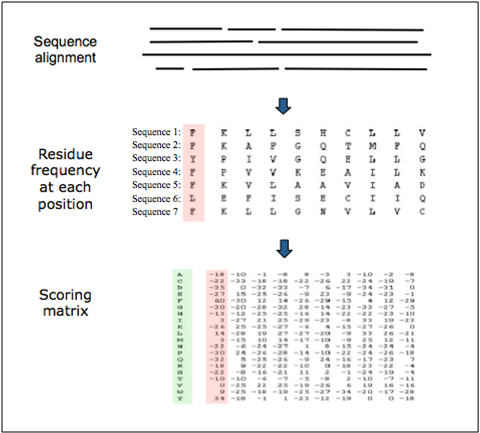
\includegraphics[width=.5\textwidth]{profile.png}
\caption{Representation of a scoring matrix based on a multiple sequence alignment. Each of the 20 amino acids commonly found in proteins is given a score for each position in the sequence according to the frequency with which they occur in the original alignment. Other factors, such as evolutionary distances can also be considered \cite{EBI}.}
\label{fig:profile}
\end{figure}

Examples of databases which use profiles to classify proteins include HAMAP and PROSITE. The PRODOM database also uses a related approach, using PSI-BLAST to create its profiles. 

\subsubsection*{Fingerprints}

Single {\em motif} methods are good at identifying features in a protein, but most protein families are characterised by not one, but several conserved regions, which occur in a certain order. Identifying these regions is the principle behind finger prints. Fingerprints are composed of multiple short conserved motifs, which are drawn from sequence alignments, as illustrated in Figure~\ref{fig:fingerprints1}. Fingerprints are used by the PRINTS database.

\begin{figure}[h!]
\centering
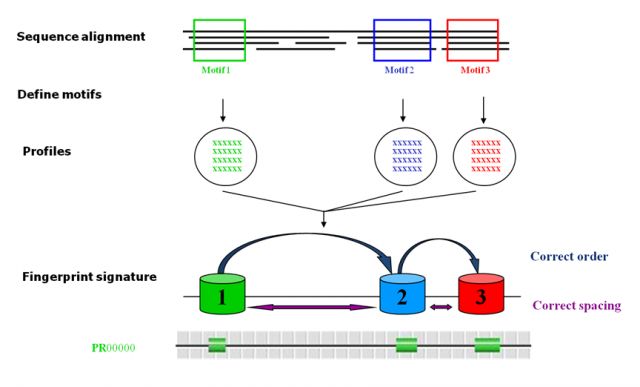
\includegraphics[width=.75\textwidth]{fingerprints1.png}
\caption{Representation of the steps involved in creating a fingerprint signature}
\label{fig:fingerprints1}
\end{figure}

Fingerprints are very good at modeling the often small differences between closely related proteins, as illustrated in Figure~\ref{fig:fingerprints2}.

\begin{figure}[h!]
\centering
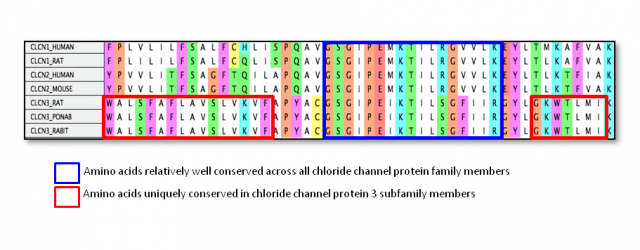
\includegraphics[width=.75\textwidth]{fingerprints2.png}
\caption{Multiple sequence alignment showing amino acid conservation across chloride channel protein family members. By using multiple short conserved motifs, fingerprints are able to distinguish closely related subfamilies from each other, such as identifying the amino acids that distinguish the chloride channel protein 3 subfamily members from other family members \cite{EBI}.}
\label{fig:fingerprints2}
\end{figure}

This means fingerprints can distinguish individual subfamilies within protein families. This allows functional characterisation of sequences at a high level of {\em specificity} (identifying individual cellular pathways in which a protein might be involved, the {\em ligand} it might bind to, the exact reaction it may catalyze, and so on). 



\subsubsection*{Hidden Markov Models (HMMs)}

Hidden Markov Models (HMMs) are like profiles in that they can convert multiple sequence alignments into position-specific scoring systems. HMMs are adept at representing {\em amino acid} insertions and deletions, meaning that they can model entire alignments, including divergent regions. They are sophisticated and powerful statistical models, very well suited for searching databases for homologous sequences. An example of how they work can be seen in Figure~\ref{fig:HMMs}. HMMs have wide utility and are used in databases such as Pfam, SMART, TIGRFAM, PIRSF, Superfamily, and Gene3D.

\begin{figure}[h!]
\centering
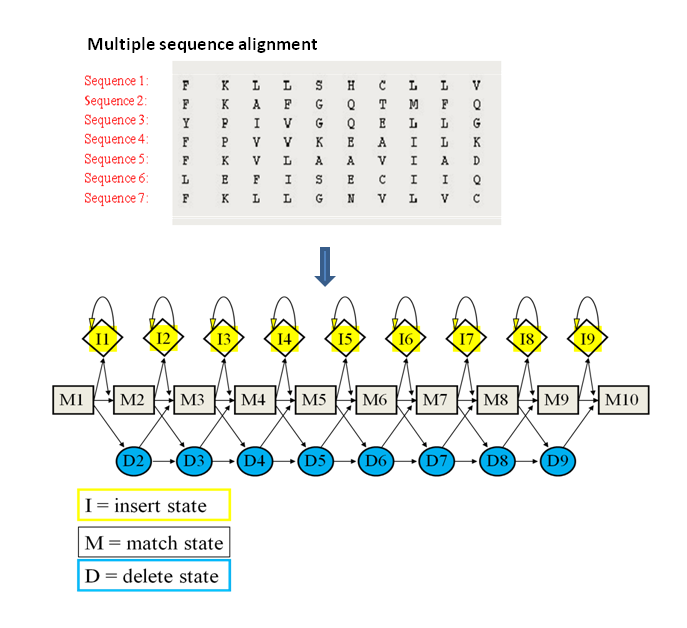
\includegraphics[width=.75\textwidth]{hmms.png}
\caption{Representation of a HMM based on a multiple alignment. Amino acids are given a score at each position in the sequence alignment according to the frequency with which they occur. Transition probabilities (i.e. the likelihood that one particular amino acid follows another particular amino acid) and insertion and deletion states are also modeled. }
\label{fig:HMMs}
\end{figure}



\section*{Algorithms}

There are quite a few algorithms that can be used for classifying these protein families. For example, the ID3 algorithm would be the most intuitive as the protein families are represented in a tree-like fashion. However, there are other methods which may run just as accurately and be more efficient, such as Markov chaining, Support Vector Machines (SVM), logistic regression, and boosted decision trees.

\subsubsection*{ID3}

Stuff about ID3

\subsubsection*{Markov chaining}

Stuff about Markov chaining

\subsubsection*{Support Vector Machines (SVM)}

Stuff about SVM

\subsubsection*{Logistic Regression}

Stuff about Logistic Regression

\subsubsection*{Boosted Decision Trees}

Stuff about boosted decision trees

\section*{Protein Data}

Specific algorithms we can use are Markov chaining or ID3. For Markov chaining we can read labeled proteins and identify common root structures. We can then count common structures to be associated to this root structure. We then can see which structures have a higher probability to attach to a domain structure. When given unlabeled proteins we can then affiliate its root domain structure to the most probable attached feature allowing us a means to label it. For the ID3 algorithm we can use the fact families of proteins have similarities in molecular sequencing. From this, and given a sufficient data base of protein sequences, we can build a decision tree which branched based on implicit sequence patterns. Available databases are SwissProt, InterPro, SCOP and the draft human genome.

\section*{Results}

\section*{Conclusion}

In conclusion, these two physics students would like you to please refer to Figure~\ref{fig:physcat}.

\begin{figure}[H]
\centering

\includegraphics{physicscat.jpg}
\caption{Don't even get us started on Computer Science}
\label{fig:physcat}
\end{figure}


\begin{thebibliography}{99}
\bibitem{EBI} European Bioinformatics Institute, "Protein Classification," \url{https://www.ebi.ac.uk/training/online/course/introduction-protein-classification-ebi/protein-classification}
\bibitem{SH3} T. Pawson and J. Schlessingert, "SH2 and SH3 Domains," Curr Biol. 1993 Jul 1;3(7):434-42
\end{thebibliography}

\end{document}
